\thispagestyle{myheadings}
\chapter{関連研究}
 本章では本研究に関連するコンテンツについての研究や生体データを用いた研究,
重畳提示手法の研究の3つのテーマについて紹介する.本研究と比較し関連性や新規性を述べる.



\section{情報媒体における研究}
 コンテンツにはたくさんの種類がある.デジタルコンテンツにはYouTubeやNetflix,
アナログコンテンツには本や新聞紙などがある.アナログコンテンツである本や新聞紙など紙で読む方がデジタルコンテンツで読むより記憶に残る研究がある\cite{books}.
スマートフォンの普及で本や新聞紙などを紙で読む機会が減った.そこで本研究のシステムを使えば,
アナログコンテンツにエフェクトを重畳し本や新聞紙を読む楽しさが増え,紙で読む機会も増えると考える.

\section{生体情報から感情を推定する研究}

 生体データを取得したときに得られる人の感情について述べる.
生体データには指紋や顔の表情など数多くの種類が存在する.
本研究では生体データを基にコンテンツにエフェクトを重畳するため,
生体データでコンテンツに対して視聴者がとる反応を抜き出す必要がある.生体データとして顔の表情から人の感情を読み取る研究がある\cite{hyoujou,hyoujou2}.
また瞳孔に注目し人が覚醒しているかを推定.人が居眠り運転するのを瞳孔を観察し事前に防ぐという研究もある\cite{doukou}.
これらの研究より生体データを使い感情が読み取れる有効性が示されている.
図のようにさまざまな生体データを用いることによって人の楽しいや辛いなどといったいくつもの感情を推定するのが可能ある.
そこで本研究ではコンテンツを視聴している時の生体データを取得し,
生体データから人の感情を読み取りコンテンツを視聴している時のどの部分が盛り上がっているポイントかを推定する.
コンテンツに対し抱いた感情をエフェクトという形で重畳し,コンテンツに新たな楽しみ方を加える.

\begin{figure}[H]
    \centering
    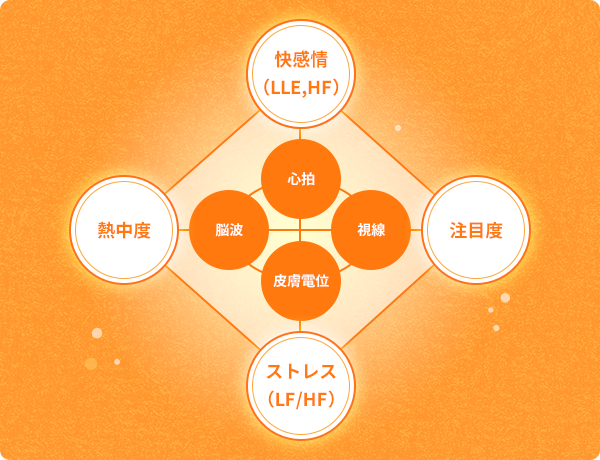
\includegraphics[width=8cm]{images/chapter2/heart.png}
    \caption{生体データからさまざまな感情を取得 : 感情体験メーケティング支援}
\end{figure}


\section{生体情報を基にフィードバックする研究}
 生体データを用いて被験者に学習支援をする研究がある\cite{seitai1,seitai2,seitai3}.生体データを使うことでより正確に支援ができるからである.
また生体情報を用いたIotも数多く存在する.生体データを活用してライフケア,ヘルスサービスの実現をしている.
例として図に示す.生体データを収集することでその人にあった適切なフィードバックが可能である.

\begin{figure}[H]
    \centering
    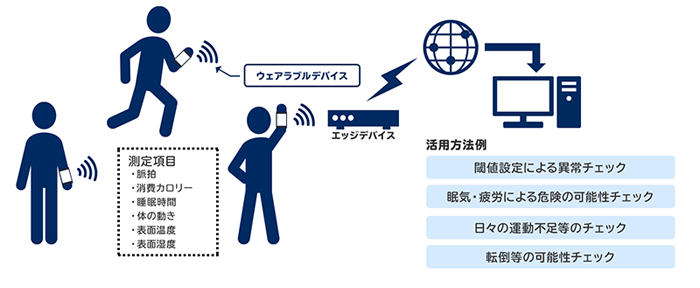
\includegraphics[width=15cm]{images/chapter2/body_img02.png}
    \caption{ウェアラブルデバイスを用いた生体情報のIot : NECソリューションイノベータ}
\end{figure}


\section{重畳提示についての研究}
コンテンツにエフェクトを重畳して面白さを増幅する研究はこれまで多くなされてきた。視線検出装置を用いてユーザがディスプレイ上の画像において任意の点に注目した際に,奥行きにフォーカスされた画像を映像に随時反映し奥行き感を強化する手法が提案されている.\cite{sityoutaikenn}\cite{hisyakaisinndo}
しかし、提案システムはあらかじめ用意した最大 256枚からなる画像を利用しており,手軽にコンテンツの視聴体験を拡張,増幅できるとは言い難く,また視線位置に応じて仮想世界のぼかし具合を変化させ,面白さや奥行き感を増幅している\cite{efects_english}.そのため本研究では重畳提示手法を使用した.

